\documentclass{article}
\usepackage[utf8]{inputenc}
\usepackage{graphicx}
\usepackage{amsmath}
\usepackage{minted}

\title{COMP 8670 - Take Home Exam}
\author{Matthew Belanger}
\date{\today}

\begin{document}

\maketitle

\section{Problem 1 - Printer Attack}

\subsection{Can Attila arrange to learn the contents of Vicky’s document without physically
accessing any of the printers?}
	\label{subsec:learn_contents}

	Yes Attila can learn the contents of Vicky's documents using a man in the middle attack 
	(assuming they are on the same network). This is possible due to two features of the protocol.
	\begin{enumerate}
		\item Attila can learn the IP addresses of all the printers on 
			the network and forward any packets recieved to the victim's requested printer. 
			This is possible due to the \textbf{Printer Discovery packets} and the \textbf{Printer Announcement packets}.
		\item Attila can recieve Vicky's print requests due to how the non-priter machines handle \textbf{Printer Announcement packets}. 
			Since \textbf{Printer Discovery packets} are broadcasted to the entire network, Attila will know when Vicky is looking for printers.
			Attila knows all the printers on the network and is able to wait a short while so the Vicky will recieve the legitimate printer data and then Attila can spoof
			additional \textbf{Printer Discovery packets} by claiming to be a printer with the same name as the actual printer,
			and when Vicky receives this new data her machine will override the entry due to the protocol specification.
	\end{enumerate}
	Due to these two possibillities, Attila can itercept Vicky's packets by pretending to be the printer and forward them to the printer and Vicky will not know the
	difference but Attila can save a copy of the sensitive data. In short, Attila learns all the names of the printers on the network, waits for discovery 
	requests and then retransmits \textbf{Printer Announcement packets} with her IP addresses but the requested printers names so that the host machines log 
	her IP as each printer on the network.
\subsection{Describe two distinct Denial-of-Service (DoS) attacks that Attila could execute
against the Printer Discovery Protocol.}
	Attila can,
	\begin{enumerate}
		\item \underline{send high volumes of \textbf{Printer Discovery packets}}, so that the printers will be unable to service legitimate
		discovery requests due to being overloaded with Attila's bogus requests.
		\item \underline{send high volumes of \textbf{Printer Announcement packets}}, so that the client machines will unable to register legitimate 
		printers requests due to being overloaded with Attila's bogus announcements.
	\end{enumerate}

\subsection{Can Attila modify what is printed on the printer?}
	Yes Attila can. See my response in section \ref{subsec:learn_contents}. Note that in the method I described, the 
	original document Vicky sends will never reach the destination printer, it is a copy that Attila forwards than reaches the printer.
	Attila can very easily swap out the document instead of forwarding a copy.

\section{Problem 2 - Hilltop Academy IT Security}
\label{sec:hilltop}

For reference, the following IP addresses are assigned based on the Hilltop Academy scenario:

\begin{align*}
    \text{Legitimate Gateway} &: \texttt{192.168.50.1} \\
    \text{Attacker (Leo)} &: \texttt{192.168.50.30} \\
    \text{Victim (Teacher)} &: \texttt{192.168.50.40} \\
    \text{Target (Internal Service)} &: \texttt{192.168.70.10}
\end{align*}

\subsection{What would be the source IP address and the MAC address in the ICMP
Redirect message sent by Leo’s Laptop to the Teacher’s Workstation?}
	Since Leo is trying to spoof the router, the IP address would need to be the gateways router so that the teacher's
	machine will believe the router is sending the information, but since Leo's the machine is physically 
	sending the packet to the teacher, it would need to be Leo's MAC address because ICMP is above the DataLink layer.

\subsection{After receiving the ICMP Redirect message, what changes occur in the routing
table of the Teacher’s Workstation?}
	The teacher will have their table updated such that it will believe that the most efficient route to get to the target machine
	will be to go to the attackers machine first.

\subsection{Indicate the new route (including the next-hop IP address) that the Teacher’s
Workstation will use to send packets intended for the Internal Web Service Server after
the ICMP Redirect attack is successful.}
	The route will begin at the source, the Teachers IP (192.168.50.40), then the Attackers IP (next hop, 192.168.50.30), then it will be the route
	to get from the attacker to the legitimate gateway and finally Internal Web Service Server 192.168.70.10.

	\[
		\text{Teacher} \xrightarrow{} \text{Leo} \xrightarrow{} \text{Gateway} \xrightarrow{} \text{Target}
	\]

\subsection{What should be the content of the ICMP Redirect message to make sure the
Teacher’s Workstation routes the traffic as intended by Leo?}
	Leo wants to just inspect the data and pass it along because Leo is not malicious. The outer message should be an IP message between
	him and the Teacher, with a redirect ICMP packet at the next layer that claims Leo is the optimal next jump. The next layer should be another IP message with
	the original information which is between the Teacher and the Target. See the Python implementation.

\subsection{If Eva notices unusual network activity and investigates the traffic coming to
and from the Teacher’s Workstation, identify the signs that would indicate an ICMP
Redirect attack is taking place.}

	Eva has not been redirected so she can ping the Teacher the "legitimate" way. Since she is on the same subnet as the Teacher she can monitor the route
	and see that the optimaml route to the target is:
	
	\[
		\text{Her} \xrightarrow{} \text{Gateway} \xrightarrow{} \text{Target}
	\]
	Leo's IP does not exist in the route, but the Teachers packet goes through Leo.
	This is evidence that some tampering has occured.

\section{Problem 3 - Python From Section \ref{sec:hilltop}}

See Python Implementation.

\section{Problem 4 - Link-State and Distance-Vector Routing}

\subsection{Assume we are using Link-State routing for the network in figure  ”Network
Topology A”. Is it possible to for oscillation problem to occur.}

\subsection{Assume we are using Distance-Vector routing for the network in figure ”Net-
work Topology A”. Is it possible to for a routing loop problem to occur.}

\subsection{Assume we are using Link-State routing for the network in figure ”Network
Topology B”. Is it possible to for oscillation problem to occur.}

\subsection{Assume we are using Distance-Vector routing for the network in figure ”Net-
work Topology B”.}

\section{Problem 5 - Congestion Control}

\subsection{Show for sending 15 different packets (duplicate packets do not count), how the
window size will change, and the packets sent in each window.}

	\begin{table}[h]
		\centering
		\begin{tabular}{cc}
			Window Size & Packets Sent \\
			1 & 1 \\
			2 & 2, 3 \\
			4 & 4, 5, 6, 7, \\
			2 & 5, 8 \\
			4 & 9, 10, 11, 12 \\
			2 & 9, 13 \\
			4 & 14, 15 \\
		\end{tabular}
		\caption{Window Size vs. Packets Sent}
		\label{tab:window_packets}
	\end{table}

\subsection{Assume that we set the initial estimated RTT to 20 ms and we measured the
actual RTT for packets 2, 5, 9, 13 as shown in table 2. Calculate the estimated RTT for
packet number 14.}

	\begin{table}[h]
		\centering
		\begin{tabular}{ccccc}
			\textbf{Packet \#} & 2  & 5  & 9  & 13 \\
			\textbf{RTT (ms)}  & 21 & 19 & 24 & 22 \\
		\end{tabular}
		\caption{Round-Trip Time (RTT) for Different Packets}
		\label{tab:rtt_data}
	\end{table}

	Given that,
	\[
		\text{EstimatedRTT}_n = (1 - \alpha) \times \text{EstimatedRTT}_{n-1} + \alpha \times \text{SampleRTT}_n
	\]

	Setting $\alpha=0.125$

	\[
		\begin{aligned}
			\text{EstimatedRTT}_2 &= (1 - 0.125) \times 20 + 0.125 \times 21 = 20.125 \\
			\text{EstimatedRTT}_5 &= (1 - 0.125) \times 20.125 + 0.125 \times 19 = 19.984 \\
			\text{EstimatedRTT}_9 &= (1 - 0.125) \times 19.984 + 0.125 \times 24 = 20.483 \\
			\text{EstimatedRTT}_{13} &= (1 - 0.125) \times 20.483 + 0.125 \times 22 = 20.676 \\
			\hline
			\text{EstimatedRTT}_{14} &= (1 - 0.125) \times \text{EstimatedRTT}_{13}  + 0.125 \times 22 = 20.841 \text{ms}
		\end{aligned}
	\]

	I use the same sample value because a new sample had not been measured so I assume the previous one is still valid.

\section{Problem 6 - TimeSync Protocol}

\subsection{Define the message format for both time synchronization requests and responses
in your protocol.}
		Before presenting a message format I want to present some considerations. A naive solution to this problem would be to create a 
		server that broadcasts the time at regular intervals and if the client sees that it has drifted then it can correct itself. \\

		Problems,
		\begin{enumerate}
			\item Does not take into account message transfer delays.
			\item How does client respond when it does not receive messages?
			\item What if client receives updates out of order? Which should it trust?
		\end{enumerate}

		It is better if the client requests the time and provides an incrementing ID of the request.\\
		In this way,
		\begin{enumerate}
			\item Still does not take into account message transfer delays.
			\item The client can re transmit the request if it does not hear anything back
			\item Reacts to the most recent ID
			% \item New problem introduced that we do not know
		\end{enumerate}

		However, we are still unsure if the message has been significantly delayed. The time server can help us with this.
		Assuming the time server has accurate knowledge of the time and that the client can accurately measure time durations, we can craft a response message that includes the accurate time along with the clients message ID so
		the client knows if the response is fresh. The client can retransmit the request if it does not hear back in 30 seconds with the same ID, thus handling time delays and packet loss. This ID is also to help the client ignore old request responses. Server should always respond to requests (Client is master, server is slave) so it does not need to 
		requests because it will be echod bach in the response.\\
		The request would be (as json),
		\begin{minted}{json}
"request": {
	"id": "uint"
}
		\end{minted}

		\begin{minted}{json}
"response": {
	"id": "uint",
	"current_time": "hh:mm:ss",
}
		\end{minted}

\subsection{Sketch a timeline for the operation of your protocol in case of a simple time
synchronization request and response with no error, and in case there is one error (e.g.
time drift greater than 30 seconds)}

	\begin{figure}[H]
		\centering
		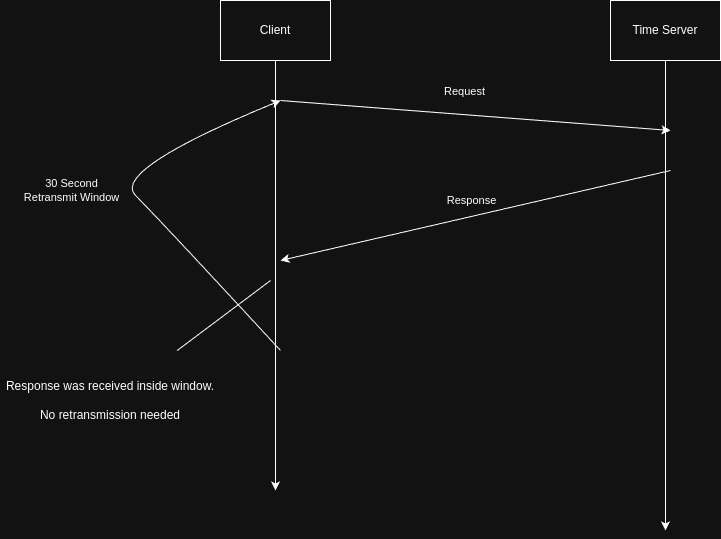
\includegraphics[width=0.8\textwidth]{no_errors.jpg}
		\caption{No Errors Diagram}
		\label{fig:no_errors}
	\end{figure}

	\begin{figure}[H]
		\centering
		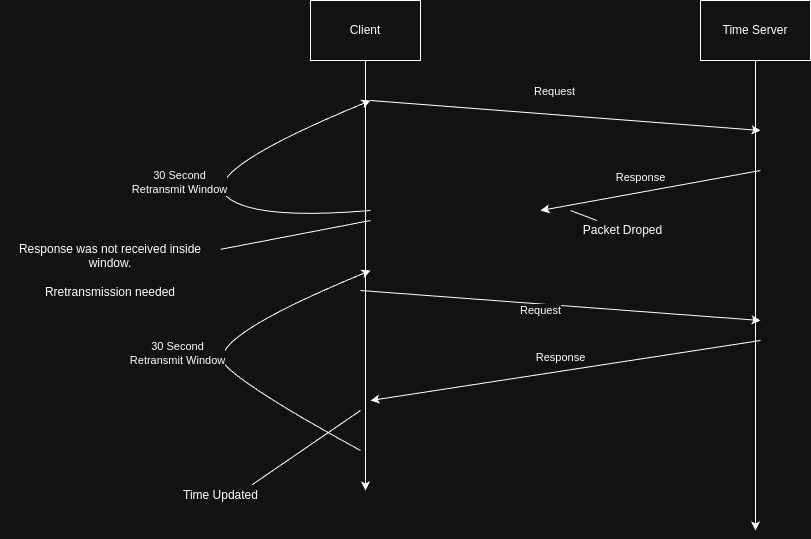
\includegraphics[width=0.8\textwidth]{one_error.jpg}
		\caption{One Error Diagram}
		\label{fig:one_error}
	\end{figure}

\section{Problem 7 - RDT Protocol}

\subsection{Draw a time chart for the packets between A and B, showing the number of
data and acknowledgment packets exchanged between A and B. When B received the
message ”CAT” correctly, there was no crash or time failure.}

\subsection{Draw a time chart for the packets between A and B, showing the number of
data and acknowledgment packets between A and B. When B only receives the message
”CA” and not ”CAT” due to time failure. A and B will fail to detect that the message
was sent incorrectly and terminate the connection.}

\subsection{Draw a time chart for the packets between A and B, showing the number of
data and acknowledgment packets between A and B. B only receives the message ”CATC”
and not ”CAT” due to time failure. A and B will fail to detect that the message was sent
incorrectly and terminate the connection.}

\end{document}
